\documentclass[rapport.tex]{subfiles}

\begin{document}
\section{Metode}
	\subsection{Metoder}
	Til dette projekt er der blevet benyttet V-modellen som udviklingmetode \cite{Vmodel}, og UML (Unified Modelling Language) \cite{UML} til design af softwarearkitekturen . V-modellen tilbyder en overskuelig tilgang til softwareudvikling i et projekt hvor en række krav er fastsat som udgangspunkt for udviklingen. Ved hjælp af UML er de forskellige krav omskrevet til use cases, og derfra er der udviklet design-diagrammer for softwarearkitekturen. 
	V-modellen følger i dette projekt følgende stadier fra analyse til implementering:
	\begin{itemize}
		\item Opstilling af krav
		\item Analyse
		\item Design
		\item Implementering
	\end{itemize}
	Disse stadier har hver endt ud i et dokument der beskriver overvejelser og arbejdet udført. \\
	
	Efter implementering af koden følger modellen en række test-stadier:
	\begin{itemize}
		\item Deltest
		\item Integrationstest
		\item Accepttest
	\end{itemize}
	
	V-modellens fleksibilitet tillader at man ved hvert teststadie kan gå tilbage og tilpasse analyse, design og implementering. 
	V-modellen giver derfor mulighed for at opstille en række krav, omskrive dem til softwarearkitektur, implementere arkitekturen, foretage tests på den implementerede kode, og derefter gå tilbage rette hvad der kunne være nødvendigt. 
	I et projekt af denne størrelse, hvor det forventes at der skal tilegnes ny viden, giver denne model derfor god mulighed for tidligt at støde på eventuelle problemer ved implementeringen, og derefter søge ny viden der kan benyttes til at opnå de opstillede krav. 
	
	\subsection{Planlægning}
	Bacheloropgaven er sat til 20 ECTS point, hvilket ifølge Aarhus Universitet svarer til 560 timer. Bachelorprojektets forløb strækker sig fra januar til slut maj, og er anslået til at vare 20 uger. Derudover har der været et forprojekt i december 2014. Der er derfor bestemt et gennemsnitligt arbejdspres på 30 timer om ugen for hele forløbet. I samarbejde med vejleder er der aftalt en times møde hver mandag. Desuden har det været bestræbt at mødes i projektgruppen hver hverdag, med forbehold for sygdom og så ledes. Internt i projektgruppen har det været aftalt af føre personlig logbog, hvori overvejelser og noter kunne føres. \\
	\\
	Tidsplan for projektet (se figur \ref{fig:Tidsplan}) er blevet udført i løbet af forprojektet med henblik på projektstruktur som angivet af v-modellen. Denne tidsplan er blevet opdateret løbende igennem projektet. 
	
	\begin{figure}
	\centering
	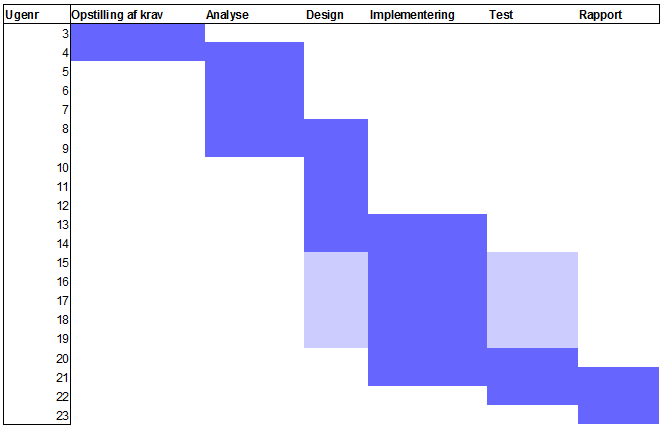
\includegraphics[width=0.9\linewidth]{Tidsplan}
	\caption{Tidsplan for projektet. Mørkeblå farve viser den konkrete tidsplan. lyseblå farve viser perioder hvor det forventedes at de forskellige stadier ville overlappe hinanden.}
	\label{fig:Tidsplan}
	\end{figure}
	
	\subsection{Diskussion}
	Har de valg vi har taget været relevante? Kort reflektion
		
\end{document}